\chapter{Models and Methods}

The models presented in chapter~\ref{relevant-models} seem to work well in the context of adaptive systems. But could the performance be further improved by taking into account the timing information of students' answers (i.e. the response times or the breaks between practices)? As was discussed in chapter~\ref{spacing-effect}, the spacing effect is observable in environments where the students have no prior knowledge. We are interested primarily in domains where the prior knowledge varies widely between students.

\section{Models Based on Timing Information}

In this chapter we discuss several models which aim at modeling students' memory with the usage of timing information of answers. There are several issues to consider beforehand:

\begin{itemize}
  \item Students have different skills and thus the rate of retention loss varies.
  \item The difficulty of items varies, some items are forgotten faster and some slower.
  \item The prior knowledge of each student is different. If the student already has the practiced item in their long term memory, the process of forgetting is much slower.
\end{itemize}

\subsection{The Extended Model}
\label{pfaet}

One possibility how to incorporate timing information into the PFA model is by changing the memory activation in prediction. The times of previous attempts are passed to a \textit{time effect function} which may increase the probability of recall (see Equation~\ref{eq-pfa-standard-time-p}).

\begin{equation} \label{eq-pfa-standard-time-p}
  P(m) = \frac{1}{1 + e^{-(m + f(t))}}
\end{equation}

Since this is an extension of the standard PFA model, it is possible to integrate the estimation of prior knowledge as well as the probability of guessing into the model.

\subsection{The Alternative Model}
\label{pfagt}

Another way of dealing with timing between attempts is by changing the decay factor $\xi$ of the model presented in chapter~\ref{pfa}. The model takes into account the order of questions, yet doesn't consider timing between student's practices of an item. This problem can be resolved by replacing the parameter $\xi$ with some time effect functions.

\begin{equation} \label{eq-pfa-gong-time-s}
  s_{i,j} = \sum_{k=1}^{n-1} y_k \cdot f(t_k)
\end{equation}

\begin{equation} \label{eq-pfa-gong-time-f}
  f_{i,j} = \sum_{k=1}^{n-1} |y_k - 1| \cdot g(t_k)
\end{equation}

Equations~\ref{eq-pfa-gong-time-s},~\ref{eq-pfa-gong-time-f} show the incorporation of the time effect function $f$ and $g$ in the model. The parameter $t_k$ represents the number of seconds that passed between the $k$-th practice and the most recent one. The weight of successes and failures is thus dependent on the ages of the prior practices.

As was discussed in the chapter~\ref{pfa}, the problem arises with multiple-choice questions. Another difficulty is the choice of a time effect function that fits the data well. The function should theoretically represent the rate at witch the effect of learning decays with the passage of time.

\section{Parameter Estimation}

The goal of the fitting procedure is to find the optimal parameters that perform well on new samples (in our case predict the student's ability to answer a question correctly). In this chapter we describe some metrics commonly used for the evaluation of predictive performance (i.e. the fitness of parameters in the model) and the principal algorithms that are suitable for parameter estimation in our case.

\subsection{Metrics}

In our case we are not only interested in the correctness of student's answers, our aim is to predict the probability of correct answer as it may indicate how well the student knows the answer. The information of student's knowledge is crucial if we don't want the student to be demotivated by overly difficult or simple questions. For this purpose the most suitable metrics are Root Mean Squared Error (see~Equation~\ref{rmse}) and Log Likelihood (see~Equation~\ref{ll})~\cite{Pelanek2015a}.

\begin{equation} \label{rmse}
  RMSE = \sqrt{\frac{\sum_{i=1}^n (p_i - y_i)^2}{n}}
\end{equation}

\begin{equation} \label{ll}
  LL = \sum_{i=1}^n y_i \log(p_i) + (1 - y_i) \log(1 - p_i)
\end{equation}

In other domains such as information retrieval or pattern recognition another type of metrics is commonly used which is based on qualitative understanding of errors~\cite{Pelanek2015a} instead of their probabilistic value. An advantage of this type of metrics is that it can be easily used in multi-classification tasks. These metrics, however depend on a chosen threshold, e.g. in case the threshold is set to $0.5$ the predictions $0.51$ and $0.98$ are classified as positive while predictions $0.49$ and $0.04$ are classified as negative.

\begin{table}[htbp]
  \centering
  \caption{Confusion matrix.}
  \begin{tabular}{ l l c c }
   \toprule[\heavyrulewidth]
   & & \multicolumn{2}{c}{\textbf{Predicted Outcome}} \\
   & & Positive & Negative \\
   \midrule[\heavyrulewidth]
   \multirow{2}{5em}{\textbf{Observed Value}}
   & Positive & True Positive (TP) & False Negative (FN) \\
   & Negative & False Positive (FP) & True Negative (TN) \\
   \bottomrule[\heavyrulewidth]
  \end{tabular}
  \label{table:confusion-matrix}
\end{table}

The Table~\ref{table:confusion-matrix} shows the confusion matrix of binary classifier (i.e. the mislabeling of classes). Once the confusion of classes is calculated, we can derivate for example precision (see~Equation~\ref{precision}) and accuracy (see~Equation~\ref{accuracy}).

\begin{equation} \label{precision}
  \mathit{Precision} = \frac{TP}{TP + FP}
\end{equation}

\begin{equation} \label{accuracy}
  \mathit{Accuracy} = \frac{TP + TN}{TP + FP + TN + FN}
\end{equation}

Even though the precision and accuracy aren't very fit in our case as we are more interested in probabilistic understanding of errors, another commonly used metric based on marking predictions as true/false positives/negatives is Area Under the ROC Curve (AUC). In this metric, we measure the performance across all possible thresholds, the result is a number between $0.5$ and $1$ where $1$ represents perfect predictions of the classifier.

\subsection{Grid Search}

This technique is used for parameter optimization, it searches a small part of the whole space of all possible values. The most fitted values are estimated using a chosen metric for evaluation (e.g. RMSE). Put together, this method exhaustively generates a grid of all combinations of selected parameter values. The fittest combination has the lowest error. The figure~\ref{fig-grid-search-rmse-auc} portrays an example of the grid search on PFA model with two parameters.

\begin{figure}[htbp]
  \centering
  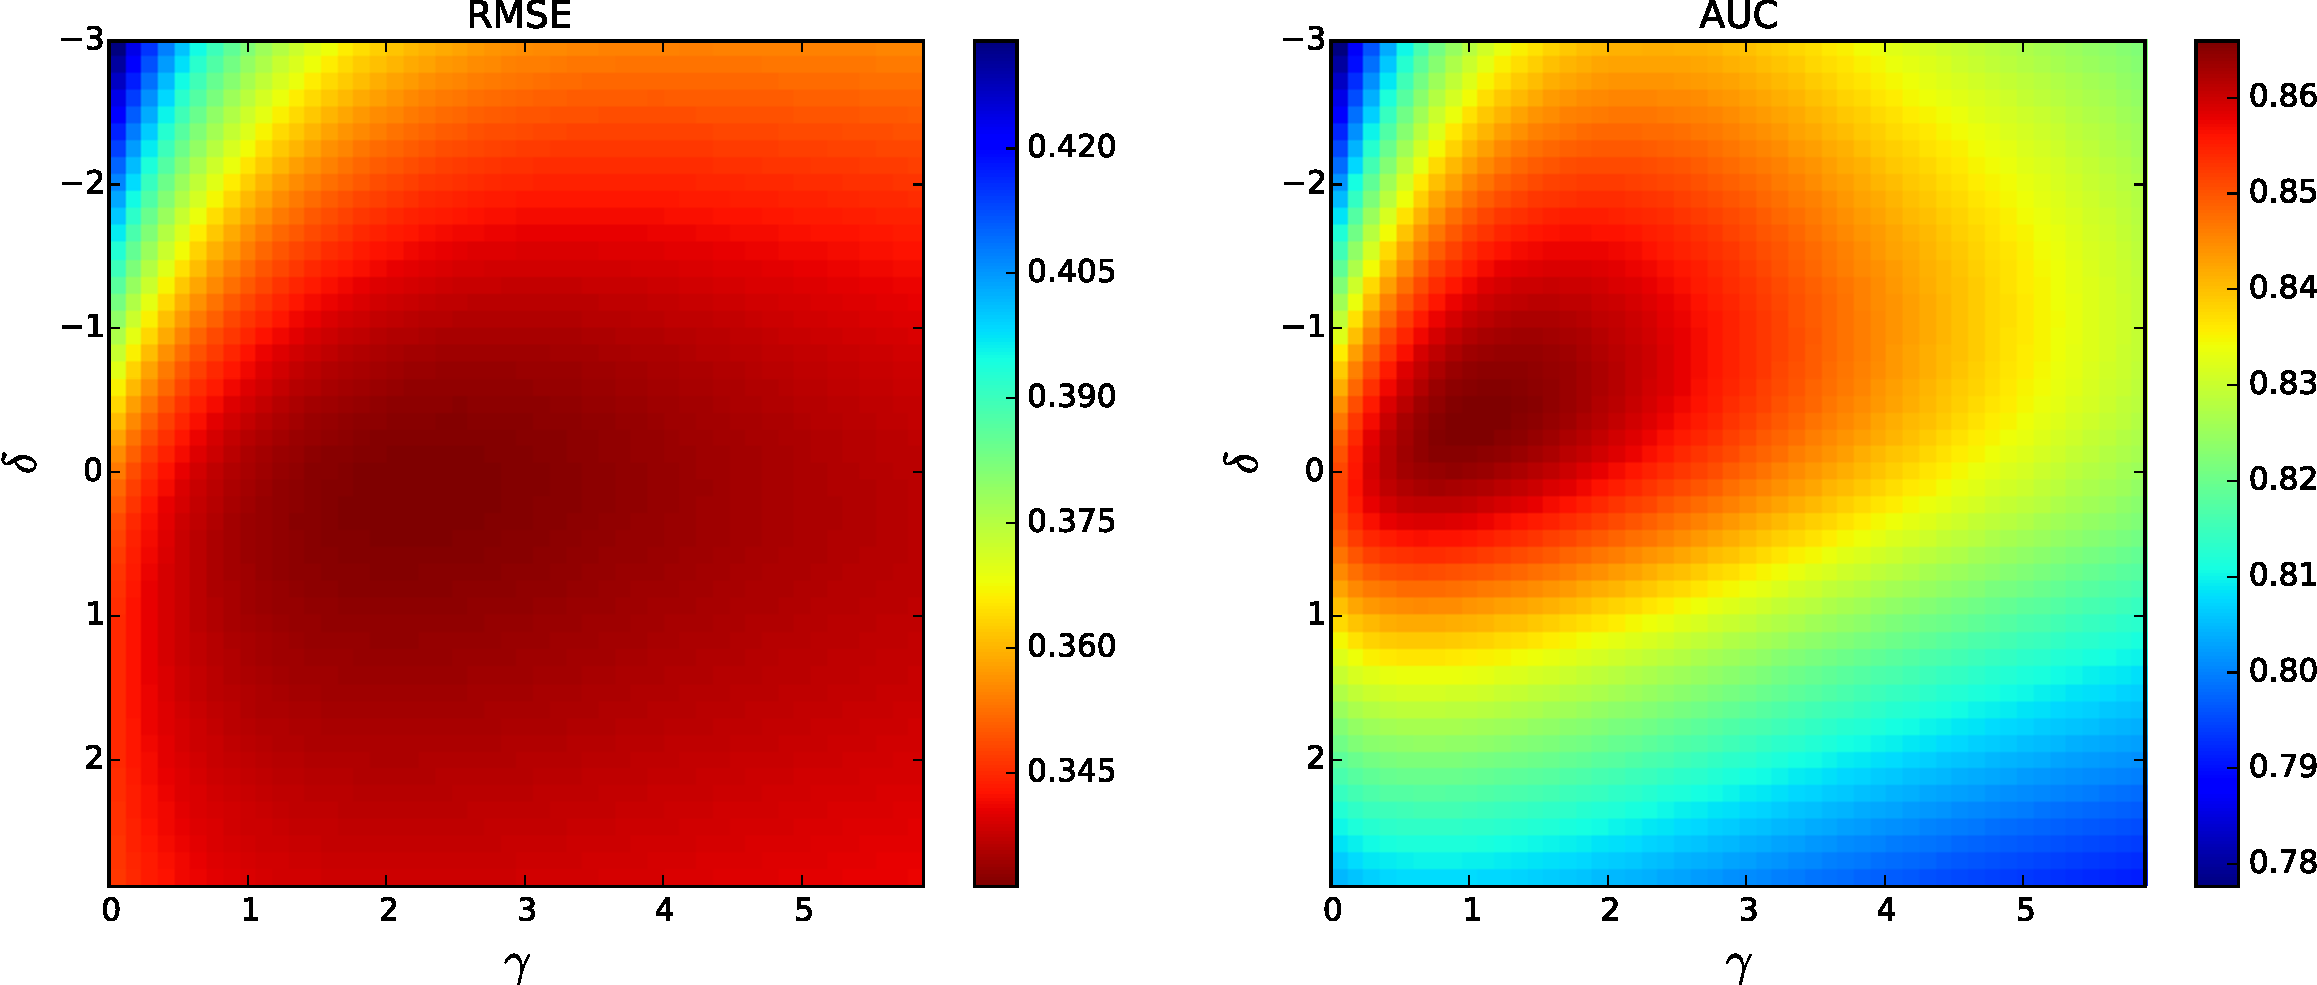
\includegraphics[width=\textwidth]{img/pfa-grid-search-rmse-auc}
  \caption{Result of the grid search performed on the PFAE model.}
  \label{fig-grid-search-rmse-auc}
\end{figure}

The disadvantage of this evaluation method is the high computational complexity which makes it very hard to use especially in cases where the model contains a lot of parameters. Another disadvantage is that when the grid is very high-dimensional we don't have any simple way to plot or visualize the error space.

\subsection{Greedy Search}
\label{greedy-search}

This method starts from a given position in the parameter space and evaluates the model's error (using some common metric). The model is then evaluated using the parameters from the enclosing neighborhood and the best option is selected. This continues until there is no other parameter value in the neighborhood with a better value. TODO: elaborate, describe the usage of randomness and decreasing size of one step.

\subsection{Gradient Descent}
\label{gradient-descent}

The goal of gradient descent algorithm is to find the best parameters for a function called hypothesis~\cite{Klusasek2014}. Gradient descent is somewhat similar to the greedy search algorithm presented in the previous section~\ref{greedy-search} as it tries to find the lowest value of the cost function $J(\rho)$. The cost function represents the error of any chosen hypothesis $h_{\rho}(x_i) = \rho^T x_i = \sum^n_{j=0} \rho_j x_{i,j}$, where $\rho_j$ is the value of the $j$-th parameter and $x_{i,j}$ the $i$-th value of the $j$-th feature (e.g. the skill of the student $i$).

\begin{equation} \label{cost-function}
  J(\rho) = \frac{1}{2m} \sum^m_{i=1} (h_{\rho}(x_i) - y_i)^2
\end{equation}

The cost function in Equation~\ref{cost-function} is the sum of all squared errors of hypotheses $h_{\rho}$ over all examples from data set of size $m$ divided by $2m$. The goal is to minimize the value of $J(\rho)$ which can be done very efficiently by the estimation of the gradient using the following update rule (TODO: elaborate):

\begin{equation} \label{cost-function-update}
  \rho_j \gets \rho_j - \alpha \frac{\partial}{\partial \rho_j} J(\rho)~~\text{for all } j
\end{equation}

The partial derivatives help indicate the surface of the cost function, it gives us the information which direction to take in order to reach the closest local minimum. The value of $\alpha$ is the size of one step or a learning rate, if the value is too big the algorithm might not be able to ever reach a local minimum, in contrast if the value is very small, it is less efficient and the computation takes longer. Now we can imagine that the main difference between gradient descent and greedy search is that the latter doesn't have any indication of which turn to take next and how big one step in a direction should be.

\begin{figure}[htbp]
  \centering
  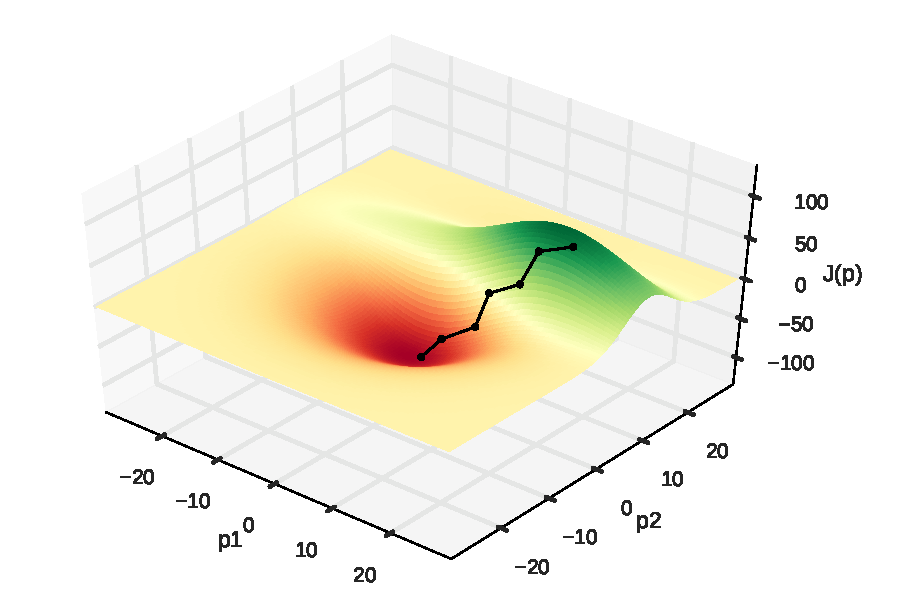
\includegraphics[width=\textwidth]{img/gradient-descent}
  \caption{3D visualization showing first 7 iterations of gradient descent applied to an example with two parameters.}
  \label{fig-gradient-descent}
\end{figure}

\subsection*{Gradient Descent in Online Learning}

In online learning, straightforward way to use optimization methods such as gradient descent doesn't exist. We can, however reuse some aspects of several algorithms used in machine learning and data mining for parameter optimization.

The most obvious and easiest way to implement gradient descent in online learning could average the difference between observation (correctness of student's answer $y_i$) and prediction (model's predicted probability that the user $i$ answers correctly $p_i$). The batch update rule similar to the one used in the original gradient descent would be defined as follows:

\begin{equation} \label{online-learning-batch-rule}
 \rho_j \gets \rho_j - \alpha~\frac{1}{n}\sum_{i=0}^n (p_i - y_i)~~\text{for all } j
\end{equation}

It is very easy to demonstrate that this method doesn't work very well even when the number of parameters is equal to 2. The parameters get easily stuck in the local minimum as can be observed in the Figure~\ref{fig-grid-search-rmse-off}.

\begin{figure}[htbp]
  \centering
  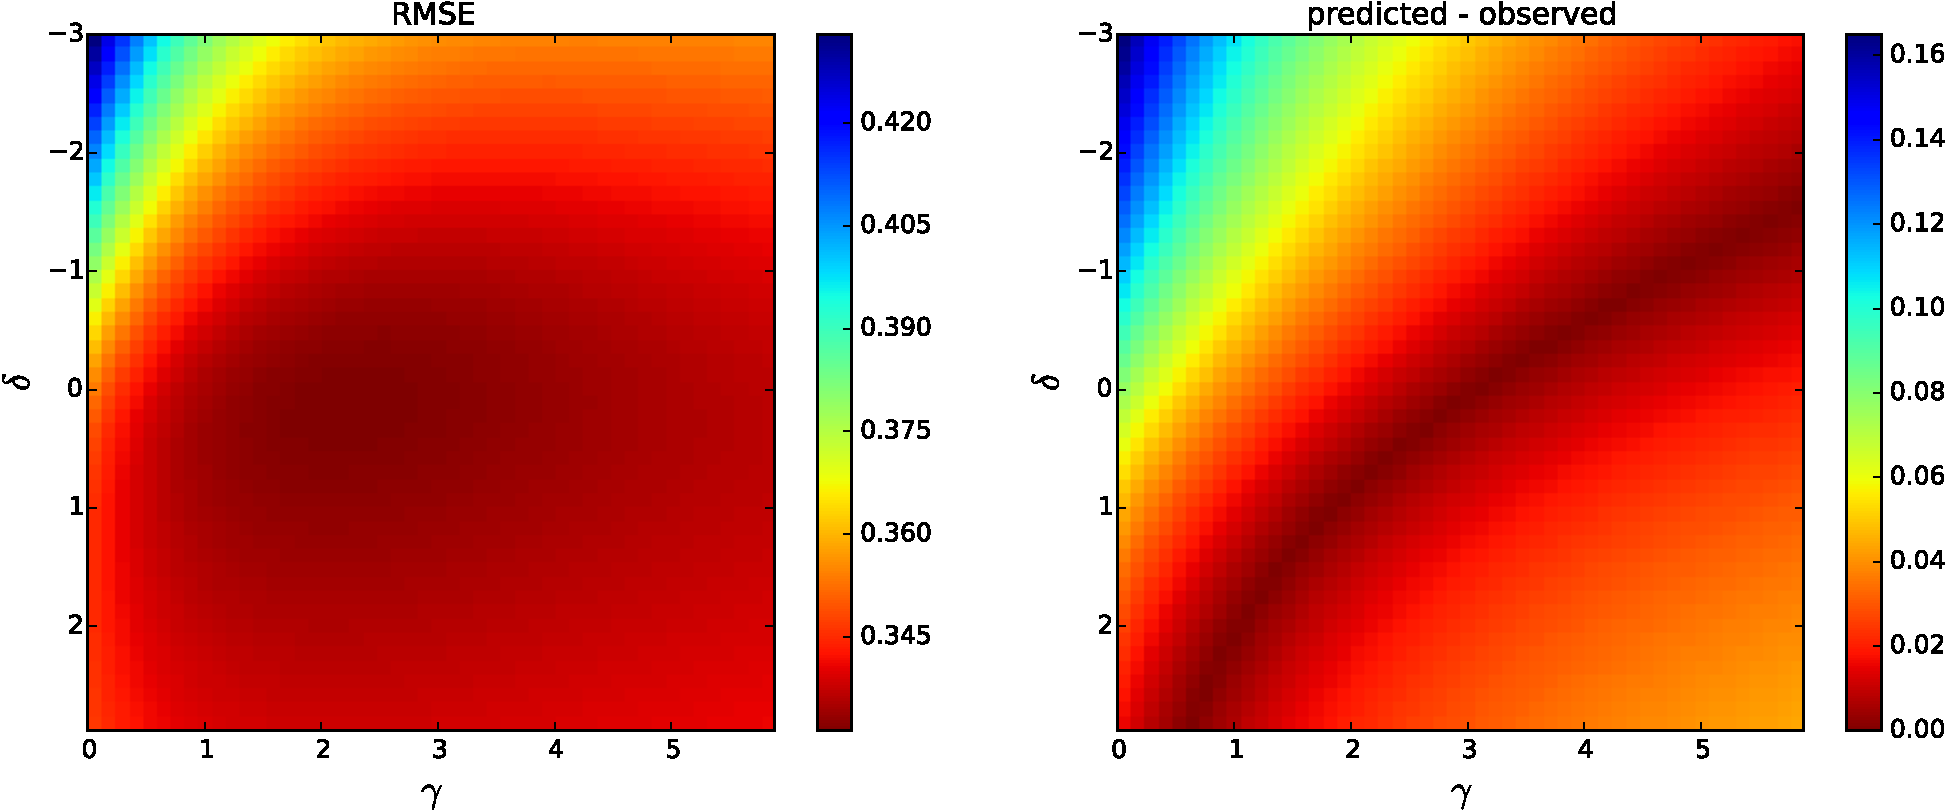
\includegraphics[width=\textwidth]{img/pfa-grid-search-rmse-off}
  \caption{Result of the grid search performed on the PFAE model with 2 parameters. The figure on the right hand size shows the averages of $p_i - y_i$ over all answers for a grid of parameters.}
  \label{fig-grid-search-rmse-off}
\end{figure}

Radek Pelánek invented a better, more complicated way of parameter fitting~\cite{Pelanek2015} that is very practical particularly in our case where we need to find the most optimal and best calibrated time effect function. (TODO: elaborate, properly describe the method and its applications)

\section{Time Effect Functions}
\label{time-effect-functions}

In chapter~\ref{memory} we mentioned that forgetting usually respects the power law, which is often true in cases where the students have no prior knowledge of the practiced material. For our purpose, we have chosen the following functions with parameter $t$ representing the time of the last presentation and two parameters $a$ and $b$:

\begin{itemize}
  \item $f(t) = a - c \cdot \log(t)$
  \item $f(t) = a \cdot e^{-c \sqrt{t}}$
  \item $f(t) = a / t^c$
\end{itemize}

Figures of each of these time effect functions with logarithmically scaled $x$-axis are depicted on Figure~\ref{fig-time-effect-functions}.

\begin{figure}[htbp]
  \centering
  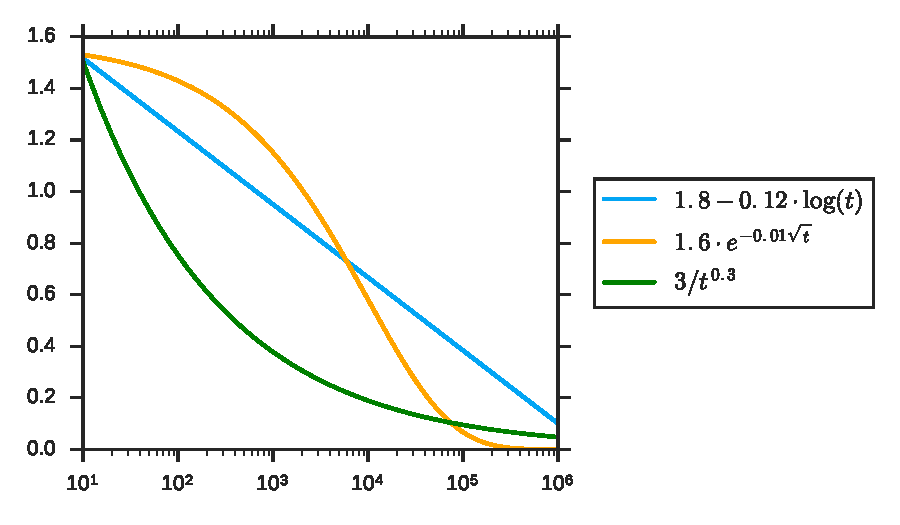
\includegraphics[width=\textwidth]{img/time-effect-functions}
  \caption{Candidates of time effect functions we inspected and evaluated in our analysis. Note that the $x$-axis is log scaled.}
  \label{fig-time-effect-functions}
\end{figure}

\subsection{The Staircase Function}
\label{staircase-function}

If we want to approximate the exact shape of time effect function, we need to define a staircase function with fixed intervals $\iota$. In each interval $(\iota_i, \iota_{i+1}]$, we preserve a learned value $a_i$ which represents an increase in memory activation. The formal definition of the staircase function $f(t)$ is formalized in Equation~\ref{eq-staircase}.

\begin{equation} \label{eq-staircase}
  f(t) = \begin{cases}
            a_1, & \text{if } \iota_0 < t \leq \iota_1 \\
            a_2, & \text{if } \iota_1 < t \leq \iota_2 \\
                 & \hspace{1em} \dots \\
            a_n, & \text{if } \iota_{n-1} < t \leq \iota_n
         \end{cases}
\end{equation}

Applying simple linear algebra, we can further modify the staircase function so that the memory activation between two points is a linear function, this makes a better approximation of the learned values. The definition of the adjusted function is described in Equations~\ref{eq-staircase-iota-prime-definiton} and~\ref{eq-staircase-linear}, where $T$ is a set of all timing distances of all answers.

\begin{equation} \label{eq-staircase-iota-prime-definiton}
\begin{split}
  \hat{\iota}_0 &= \iota_0 \\
  \hat{\iota}_i &= \mathit{mean}\{t \in T~|~\iota_{i-1} < t \leq \iota_i\}
\end{split}
\end{equation}

\begin{equation} \label{eq-staircase-linear}
  f(t) = \begin{cases}
            a_1, & \text{if } \hat{\iota}_0 < t \leq \hat{\iota}_1 \\
            (t - \hat{\iota}_1) \frac{a_2 - a_1}{\hat{\iota}_2 - \hat{\iota}_1} + a_1, & \text{if } \hat{\iota}_1 < t \leq \hat{\iota}_2 \\
            \hspace{9em} \dots \\
            (t - \hat{\iota}_{n-1}) \frac{a_n - a_{n-1}}{\hat{\iota}_n - \hat{\iota}_{n-1}} + a_{n-1}, & \text{if } \hat{\iota}_{n-1} < t \leq \hat{\iota}_n     
         \end{cases}
\end{equation}

Note that $\hat{\iota}_0$ is in our case always equal to $0$ and $\hat{\iota}_n$ to infinity (in which case the memory activation in the interval is equal to $a_n$).
